\documentclass{beamer}

\usefonttheme{professionalfonts} % using non standard fonts for beamer
\usefonttheme{serif} % default family is serif

%\usepackage{hyperref}

%\usepackage{minted}

\usepackage{animate}

\usepackage{graphicx}

\def\Put(#1,#2)#3{\leavevmode\makebox(0,0){\put(#1,#2){#3}}}

\usepackage{color}

\usepackage{tikz}

\usepackage{amssymb}

\usepackage{enumerate}


\newcommand\blfootnote[1]{%

  \begingroup

  \renewcommand\thefootnote{}\footnote{#1}%

  \addtocounter{footnote}{-1}%

  \endgroup

}

\makeatletter

%%%%%%%%%%%%%%%%%%%%%%%%%%%%%% Textclass specific LaTeX commands.

 % this default might be overridden by plain title style

 \newcommand\makebeamertitle{\frame{\maketitle}}%

 % (ERT) argument for the TOC

 \AtBeginDocument{%

   \let\origtableofcontents=\tableofcontents

   \def\tableofcontents{\@ifnextchar[{\origtableofcontents}{\gobbletableofcontents}}

   \def\gobbletableofcontents#1{\origtableofcontents}

 }

%%%%%%%%%%%%%%%%%%%%%%%%%%%%%% User specified LaTeX commands.

\usetheme{Malmoe}

% or ...

\useoutertheme{infolines}

\addtobeamertemplate{headline}{}{\vskip2pt}



\setbeamercovered{transparent}

% or whatever (possibly just delete it)

\makeatother

\begin{document}
\title[DDCEL report]{A Scalable DCEL implementation}
\author[AC]{Andres Calderon}
\institute[Spring'20]{University of California, Riverside}
\makebeamertitle
\newif\iflattersubsect

\AtBeginSection[] {
  \begin{frame}<beamer>
    \frametitle{Outline} 
    \tableofcontents[currentsection]  
  \end{frame}
  \lattersubsectfalse
}

\AtBeginSubsection[] {
  \begin{frame}<beamer>
    \frametitle{Outline} 
    \tableofcontents[currentsubsection]  
  \end{frame}
}

\begin{frame}{gadm dataset}
    \begin{itemize}
        \item Level 1 (States) and level 2 (Counties) globally.
        \item 110K and 170K polygons.
        \item 1.0G and 1.2G.
    \end{itemize}
\end{frame}

\begin{frame}{Cells}
  \centering
    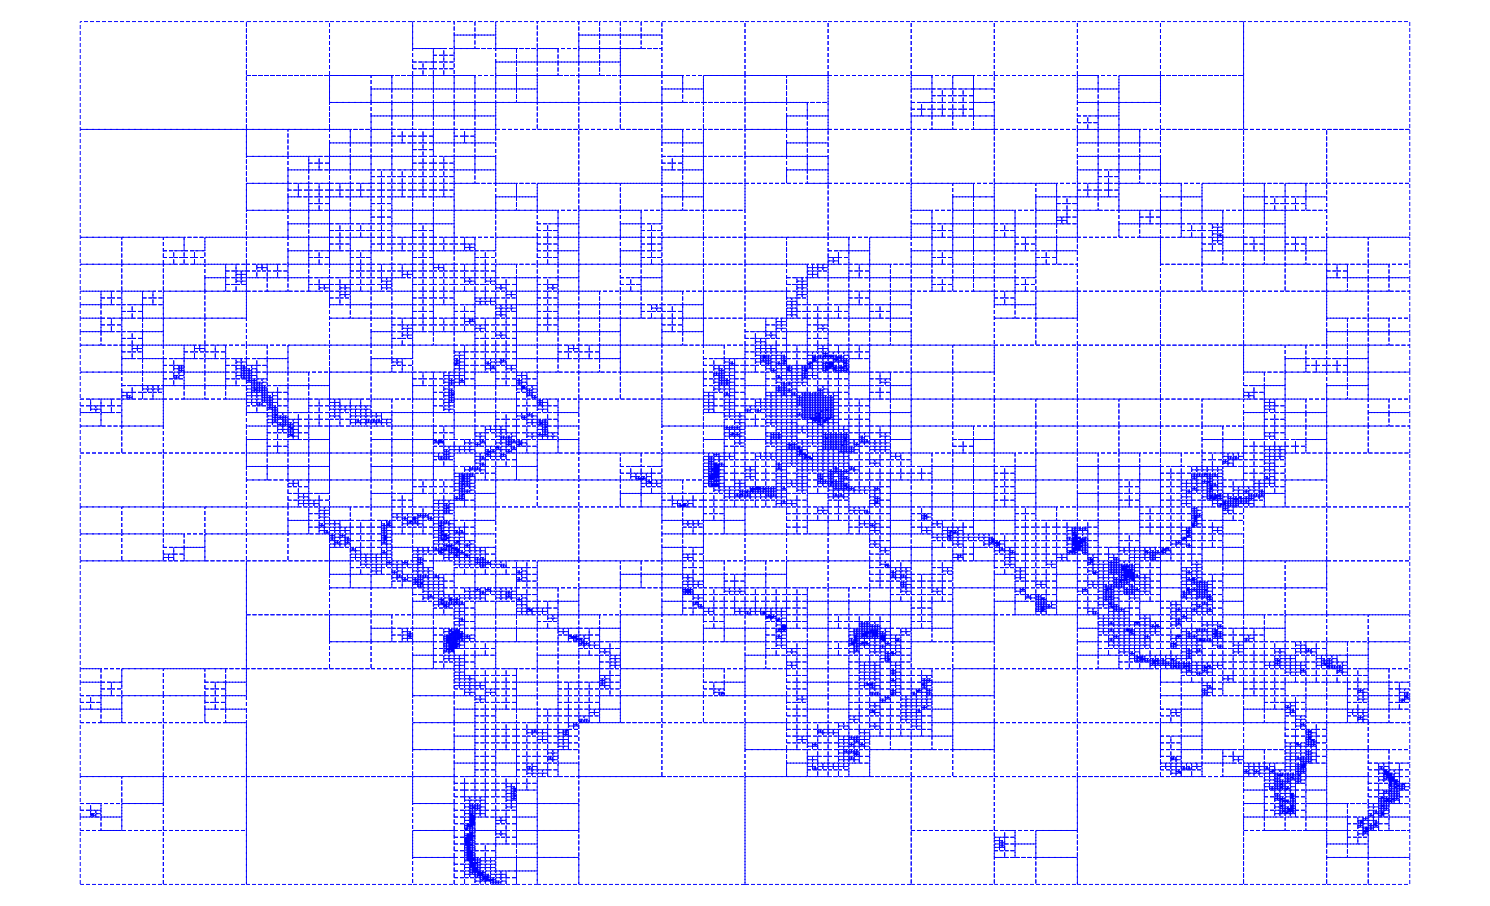
\includegraphics[width=\textwidth]{figures/gadm_grid}
\end{frame}

\begin{frame}{DCEL construction}
    \begin{itemize}
        \item Partitioning (12583 cells) in $\approx$121s. 
        \item 37.6M (level 1) and 54M (level 2) edges processed.
        \item DCEL A in $\approx$ 123s.
        \item DCEL B in $\approx$ 132s.
    \end{itemize}
\end{frame}

\end{document}
